\section{Einleitung}\label{einleitung}
Moderne Simulationen sind in der Lage grosse Mengen an Daten zu produzieren. Die rohe Datenmenge ist oft zu gross um sie zu archivieren oder in vernünftiger Zeit über eine Internetverbindung zu übertragen. In wissenschaftlichen Simulationen werden natürliche Phänomene wie Schwingungen, Flugbahnen, Kraftfelder etc. als Menge von Kurven im dreidimensionalen Raum abgebildet. Die Kurven sind dargestellt als Folge von Punkten. Ziel dieser Arbeit ist es eine verlustbehaftete Kompression für die Punktfolgen zu entwickeln, welche die Übertragung über eine Internetverbindung und die lokale Zwischenspeicherung ermöglicht.

Im Rahmen dieses Projekts werden Daten von Magnetfeldlinien der Sonne komprimiert, welche über eine Internetverbindung zum JHelioviewer übertragen werden. Der JHelioviewer ist eine Applikation zur visualisierung von Satellitenmessdaten und Simulationen der Sonne. Die Applikation wird von der ESA und der FHNW entwickelt. Die Abbildung \ref{einleitung::feldlinien} zeigt eine Visualisierung des JHelioviewers von der Sonnenoberfläche und Feldlinien.\\
\begin{figure}[!htbp]
\center
	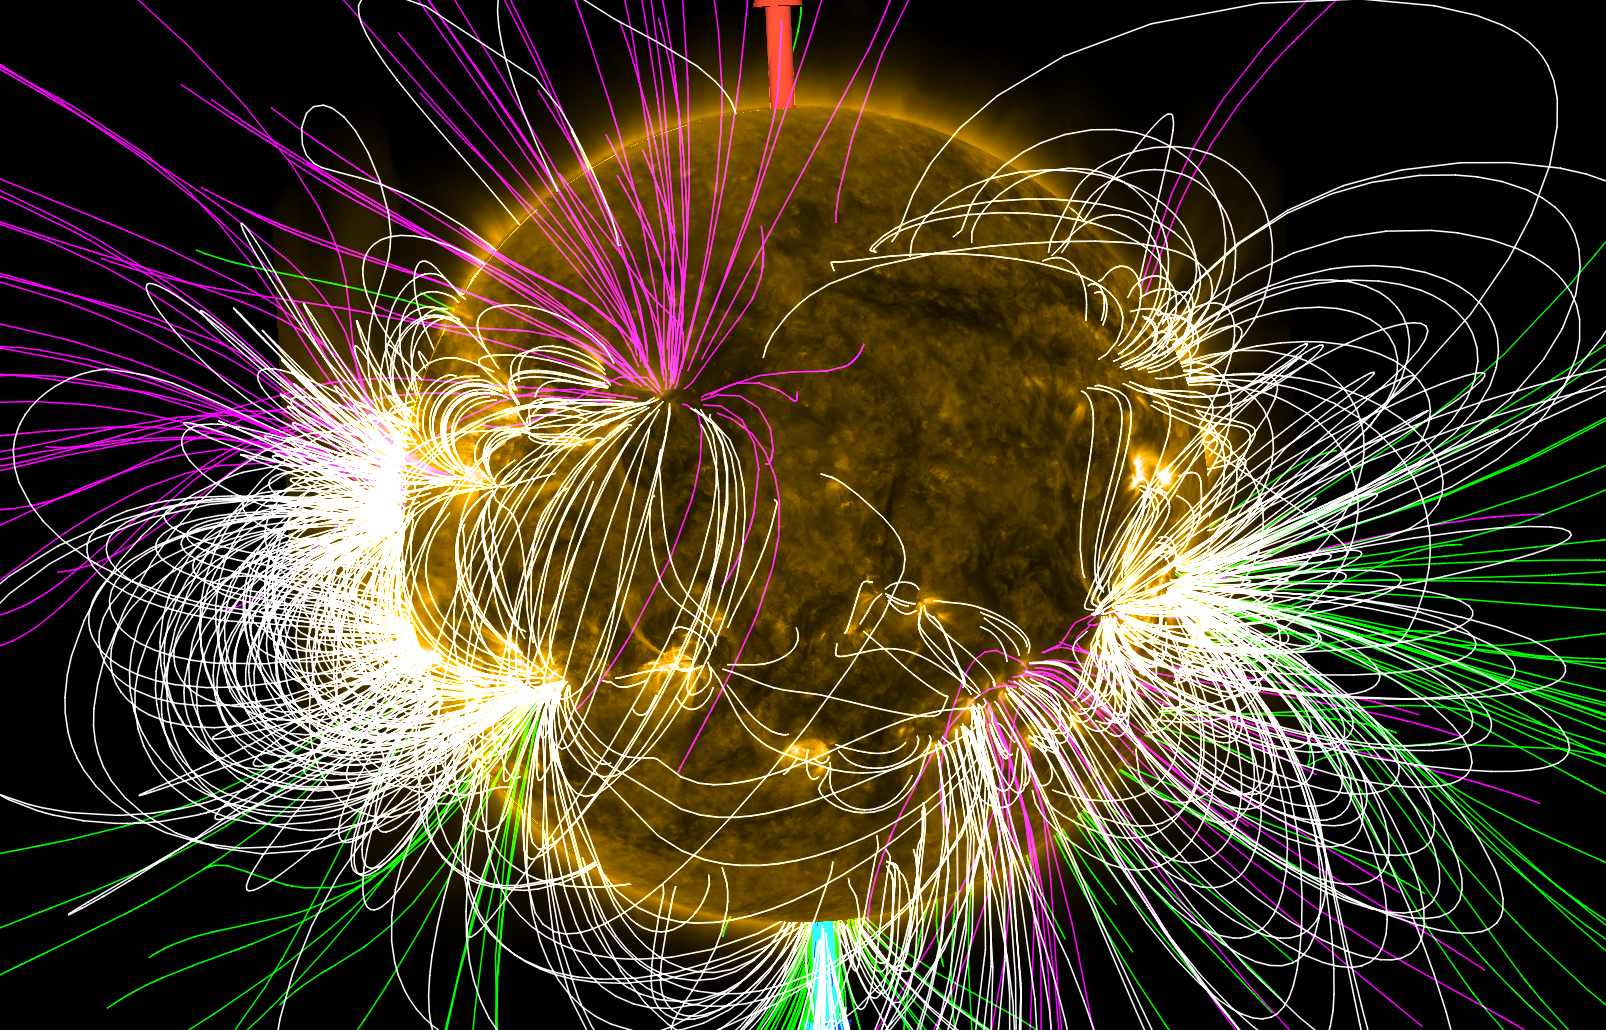
\includegraphics[width=0.8\textwidth,height=8cm,keepaspectratio]{./pictures/einleitung/fieldLines.png}
	\caption{Visualisierung der Feldlinien im JHelioviewer}
	\label{einleitung::feldlinien}
\end{figure}
Auf der Visualisierung sind Feldlinien in drei unterschiedlichen Farben zu erkennen, welche drei unterschiedle Typen darstellen: Linien, die auf der Sonne starten und wieder auf der Sonne landen, auf der Sonne starten und ins Weltall führen oder vom Weltall auf der Sonne landen. Die weissen Feldlinien repräsentieren ''Sonne zu Sonne´´, die Grünen ''Sonne ins Weltall´´ und die Violetten ''Weltall zur Sonne´´.

Der JHelioviewer ist in der Lage Abfolge von Mess- und Simulationsdaten als Animation zu visualisieren. Die Daten für die Animation werden entweder on-the-fly heruntergeladen oder zuvor im Arbeitsspeicher gecached. Im Extremfall werden $1000$ komprimierte Simulationen im Arbeitsspeicher zusammen mit anderen Mess- und Simulationsdaten abgelegt. Im Vorfeld wurde bereits eine verlustbehaftete Kompression entwickelt, welche die Datenmenge auf durchschnittlich 1 Megabyte pro Simulation reduziert. Das Caching von $1000$ Feldlinien-Simulationen benötigt im Ist-Zustand durchschnittlich ein Gigabyte an Arbeitsspeicher. Das Ziel der Arbeit ist eine verlustbehaftete Kompression zu entwickeln, welche für das Caching $1000$ Simulationen um den Faktor $8$ bis $10$ weniger Arbeitsspeicher benötigt.\\
Zusätzlich soll erforscht werden unter welchen Bedingungen und Kompromisse das on-the-fly Herunterladen von Simulationen möglich ist. Für die Animation der Feldlinien werden im Allgemeinen 1 bis maximal 10 Simulationen in der Sekunde benötigt. Ein Fernziel des JHelioviewers ist die kontinuierliche Animation der Feldlinien. Im Ist-Zustand ist jeder Wechsel der Simulation markant. Eine Möglichkeit das Ziel zu erreichen ist die Kadenz zu erhöhen und 10-30 Simulationen in der Sekunde zu animieren.

Im laufe des Projekts wurden drei Kompressionen entwickelt. Die Kompressionsraten sind der Tabelle \ref{einleitung:tabelle} ersichtlich.
\begin{table}[!htbp]
	\center
	\begin{tabular}{r|l}
		Lösungsansatz & Kompressionsrate \\\hline
		Ist-Zustand & 1\\
		Adaptives Subsampling & 11.6 \\
		Diskrete Kosinus Transformation & 14.1 \\
		Prediktive Kodierung & 13.4\\
	\end{tabular}
	\caption{Kompressionsraten der Lösungsansätze.}
	\label{einleitung:tabelle}
\end{table}